\documentclass[11pt, letterpaper]{article}
\usepackage[utf8]{inputenc}
\usepackage[letterpaper, margin=0.5in]{geometry}
\usepackage{amsmath}
\usepackage{amssymb}
\usepackage{amsthm}
\usepackage{graphicx}
\usepackage{listings}
\usepackage[font=scriptsize]{caption}
\usepackage{subcaption}
\usepackage{xcolor}

\newtheorem{lemma}{Lemma}
\newcommand{\indep}{\perp \!\!\! \perp}

\definecolor{codegreen}{rgb}{0,0.6,0}
\definecolor{codegray}{rgb}{0.5,0.5,0.5}
\definecolor{codepurple}{rgb}{0.58,0,0.82}
\definecolor{backcolour}{rgb}{0.95,0.95,0.92}

\lstdefinestyle{mystyle}{
    backgroundcolor=\color{backcolour},   
    commentstyle=\color{codegreen},
    keywordstyle=\color{magenta},
    numberstyle=\tiny\color{codegray},
    stringstyle=\color{codepurple},
    basicstyle=\ttfamily\footnotesize,
    breakatwhitespace=false,
    texcl=true,
    mathescape=true,
    breaklines=true,                 
    captionpos=b,                    
    keepspaces=true,                 
    numbers=left,                    
    numbersep=5pt,                  
    showspaces=false,                
    showstringspaces=false,
    showtabs=false,                  
    tabsize=2
}

\lstset{style=mystyle}
\graphicspath{ {.} }
\captionsetup{justification=raggedright, singlelinecheck=false}

\author{Ryan Tang}
\title{STA 542 HW 3}
\date{March 6th 2023}

\begin{document}
\maketitle

\section{Ex 1}
First, we plot a simple cosine harmonic series, f(t), $2\pi$ periodic at a 200 sampling rate for 5 seconds. In other words, $f(t)$ has $\lambda = 200$ wavelength. Then, we plot $g(t)=|f(t)|$ right next to it both in the time and frequency domain. We notice a few things.
\begin{itemize}
    \item $g(t)$ is no-longer $2\pi$ periodic.
    \item The power spectrum of $g(t)$ has a value on every 10-th interval that decays off exponentially. 
\end{itemize}

The first item is obvious because we are taking an absolute of the original symmetric function around 0. Hence, we should expect at least double the frequency. The latter is more subtle. It has more to do with $g(t)$'s sharp turn on point zero. To fit it using cosine and sine requires an infinite number of them --- Gibbs phenomena.

\begin{figure*}[!h]
  \centering
  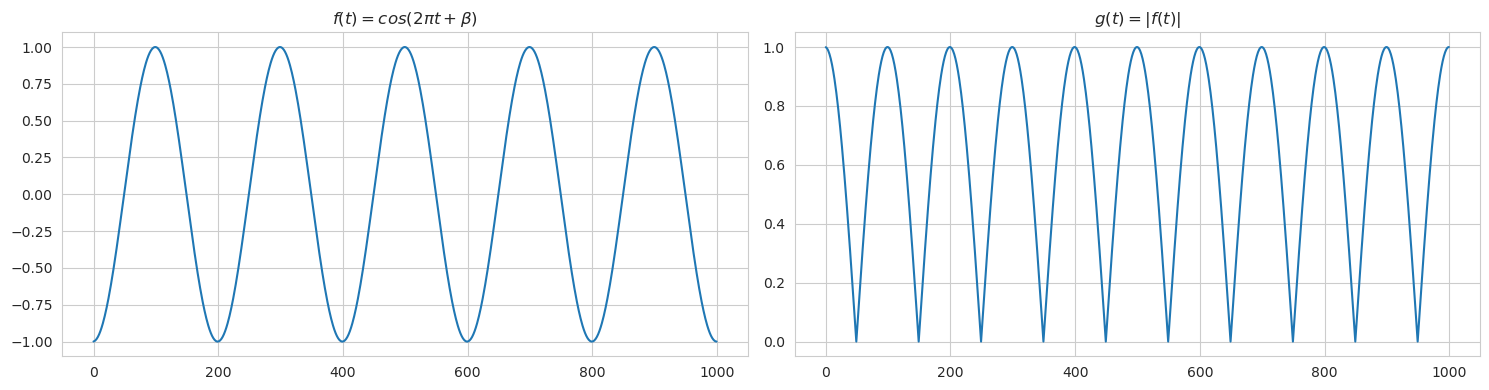
\includegraphics[width=1.0\textwidth]{1-1.png}
  \captionsetup{justification=centering}
  \caption{Comparison in the time domain}
\end{figure*}

\begin{figure*}[!h]
  \centering
  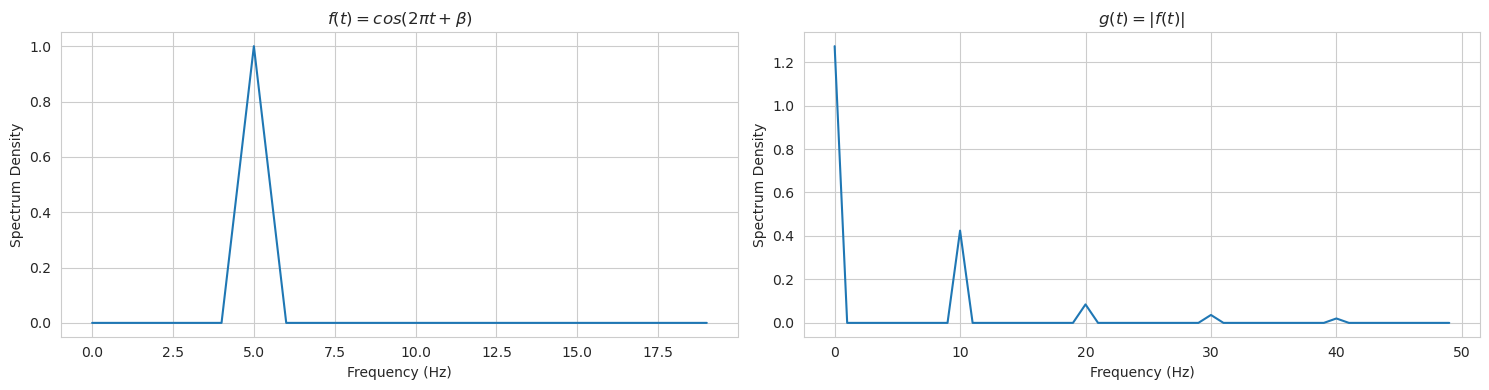
\includegraphics[width=1.0\textwidth]{1-2.png}
  \captionsetup{justification=centering}
  \caption{Comparison in the frequency domain}
\end{figure*}

 \newpage
\section{Ex 2}
Using the Yule-Walker equations, we can have the following.
\begin{align*}
    \hat{\phi_2} &= \hat{\Gamma}_2^{-1} \gamma_2 \\
        &= \begin{bmatrix}\gamma(0) & \gamma(1) \\ \gamma(1) & \gamma(0)\end{bmatrix}^{-1} \begin{bmatrix}\gamma(1) \\ \gamma(2)\end{bmatrix} \\
        &= \begin{bmatrix}1382.2 & 1114.4 \\ 1114.4 & 1382.2\end{bmatrix}^{-1} \begin{bmatrix}1114.4 \\ 591.72\end{bmatrix} \\
        &= \begin{bmatrix}1.318 \\ -0.634\end{bmatrix} \\
    \hat{\sigma^2} &= \gamma(0) - \hat{\phi_2}^{\intercal} \gamma_2 \\
        &= 1382.2 - \begin{bmatrix}1.318 & -0.634\end{bmatrix} \begin{bmatrix}1114.4 \\ 591.72\end{bmatrix} \\
        &= 289.166
\end{align*}
Lastly, since we are considering Gaussian AR(p=2) process, the Yule-Walker estimators follows $\hat{\phi}-\phi \xrightarrow{p} N(0, \frac{\sigma^2}{n}\Gamma_2^{-1})$ asymptotic convergence to normal. Hence, the estimation variances are below, which are reduced proportionally to the number of observations n.
\begin{align*}
    \sigma^2\Gamma_2^{-1} &= \begin{bmatrix}0.597 & -0.482 \\ -0.482 & 0.597\end{bmatrix} \\
    CI(\hat{\phi}, q=0.95) &= \begin{bmatrix}1.318 \\ -0.634\end{bmatrix} \pm 1.96 * \sqrt{0.597/n}
\end{align*}

\section{Ex 3}
Using the provided sample covariances, we apply the Durbin-Levison Recursion to obtain the $\hat{\phi}$ at each step.
\begin{align*}
    \hat{\phi}_{11} &= [0.806]' \\
    \hat{\phi}_{22} &= [1.318, -0.634]' \\
    \hat{\phi}_{33} &= [1.369, -0.740, 0.081]' \\
\end{align*}
Then, the corresponding PACF coefficients asymptotically converge in distribution to Gaussian under the casual AR(p) assumption, $\sqrt{n}\hat{\phi}_{hh} \xrightarrow{d} N(0,1)$. Hence, the 3-rd order coefficient has the 95-the confidence interval $0.081 \pm 1.96/\sqrt{n}$. In other words, we need at least a 585 sample size to claim the statistical significance for the 3-rd order coefficient.

\section{Ex 4}



\end{document}